% Chapter 3

\chapter{Literature Review} % Main chapter title

\label{review} % For referencing the chapter elsewhere, use \ref{Chapter1} 

\lhead{Chapter 3. \emph{Literature Review}} % This is for the header on each page - perhaps a shortened title

\section{Event Identification in News Text}
The event detection task \cite{allan2002topic} in the TDT program (Topic Detection and Tracking), led to significant advancements in the field of event-based organization of broadcast news. Some of the efforts in the TDT program focused on online event detection from continuous and real-time streams of textual news documents in newswires \cite{allan1998line,kumaran2004text}. While others explored the detection of past events from archived news documents \cite{yang1998study}. 

The textual content in news documents are different from the short informal text common in the realm of social media.  Most of these documents contain formal text with well-formed grammatical structures, enabling the researchers to rely on the state-of-the-art natural language processing techniques. Named entity extraction and Parts-of-Speech (POS) tagging are among the widely used techniques. Zhang et al. \cite{zhang2007new} extracted named entities and POS tags from textual news documents, and used them to reweigh tf-idf representations of these documents for the new event detection task. Filatova and Hatzivassiloglou \cite{hatzivassiloglou2003domain} identified named entities corresponding to participants, locations, and times in text documents, and then used the relationships between certain types of entity pairs to detect event content. Hatzivassiloglou et al. \cite{hatzivassiloglou2000investigation} used linguistic features (e.g., noun phrase heads, proper names) and learned a logistic regression model for combining these features into a single similarity value. Makkonen et al. \cite{makkonen2004simple} extracted meaningful semantic features such as names, time references, and locations, and learned a similarity function that combines these metrics into a single clustering solution. They concluded that augmenting documents with semantic terms did not improve performance, and reasoned that inadequate similarity functions were partially to blame. 

Extracting events from text has been the focus of numerous studies as part of the NIST initiative for Automatic Content Extraction (ACE) \cite{ahn2006stages,ji2008refining}. The ACE program defines event extraction as a supervised task, given a small set of predefined event categories and entities, with the goal of extracting a unified representation of the event from text
via attributes (e.g., type, subtype, modality, polarity) and event roles (e.g., person, place, buyer, seller). Ahn \cite{ahn2006stages} divided the event extraction task into different subtasks, including identification of event keyword triggers (see Chapter 2), and determination of event
coreference, and then used machine learning methods to optimize and evaluate the results of each subtask. Ji and Grishman \cite{ji2008refining} proposed techniques for extracting event content from multiple topically similar documents, instead of the traditional approach of extracting events from individual documents in isolation. In contrast with the predefined templates outlined by ACE, Filatova et al. \cite{filatova2006automatic} presented techniques to automatically create templates for event types, referred to as domains, given a set of domain instances (i.e., documents containing information related to events that belong to the domain). 

As already discussed, social media documents are extremely concise, noisy and lacks well-established grammatical structures. Therefore, the techniques used in these works are not suitable for identification of events from social media.  It has been shown that it is extremely challenging for the state-of-the art information extraction algorithms to perform efficiently and give accurate results for micro-blogs \cite{derczynski2013microblog}. For example, named entity recognition methods typically show 85-90\% accuracy on longer texts, but 30-50\% on tweets \cite{ritter2011named}. Therefore, new approaches had to be taken, leading to new techniques for detecting events in social media, which we discuss next.

%One of the goals of the EIIM framework presented in this thesis, is to identify and track event related content being generated in social media. However, the framework does not require detection of unknown events from real-time streams of social media messages. Instead it is provided with a predefined set of events along with predefined hashtags for the respective events, which are used for relevant data collection.

\section{Event Identification in Social Media}
While event detection in textual news documents has been studied in depth, the identification
of events in social media sites is still in its infancy. Several related papers explored the unknown event identification scenario in social media.
Weng and Lee \cite{weng2011event} proposed wavelet-based signal detection techniques for identifying
real-life events from Twitter. These techniques can detect significant bursts or trends
in a Twitter data stream. Sankaranarayanan et al. \cite{sankaranarayanan2009twitterstand}
identified late breaking news events on Twitter using clustering, along with a text-based
classifier and a set of handpicked news seeders. But they do not take into account the filtering of non-event content, which results in poor performance. Segregating the messages that have high likelihood of containing informative content from the ones with chances of having non-informative content are at the core of our work.  

% but, unlike our work in Chapter 4, they do not filter the vast
%amount of non-event content that exists on Twitter. This, unfortunately, results in poor
%performance, with very low precision scores compared with the precision achieved by our
%methods. Related to our work in Chapters 4 and 5, 



%As we discussed, such text-based and seeder-driven filtering of
%non-event data can be used to generate the event document stream we use in Chapter 5.

Petrovic et al. \cite{petrovic2010streaming} used locality-sensitive hashing to detect the first tweet associated with an event in a stream of Twitter messages. Rattenbury et al. \cite{rattenbury2007towards} analyzed the temporal usage distribution of tags to identify tags that correspond
to events. Chen and Roy \cite{chen2009event} used the time and location associated with Flickr image
tags to discover event-related tags with significant distribution patterns (e.g.bursts) in
both of these dimensions.
 
%
%%We use the general text-based classifier suggested in \cite{sankaranarayanan2009twitterstand} and a method for identifying top events suggested by Petrovic et
%%al. \cite{petrovic2010streaming} as baseline approaches in our evaluation of the unknown identification methods
%%of Chapter 4. While our work in the unknown event identification scenario focuses on timely, online, analysis, several efforts tried to address this task using retrospective analysis. 


Recent efforts proposed techniques for known identification of events in social media.
Many of these techniques rely on a set of manually selected terms to retrieve event-related
documents from a single social media site \cite{sakaki2010earthquake,yardi2010tweeting}. Our method of tracking an event is similar to this. We also use predefined hashtags to bootstrap the process of collecting data related to a known set of events. Sakaki et al. \cite{sakaki2010earthquake} developed
techniques for identifying earthquake events on Twitter by monitoring keyword triggers
(e.g., earthquake or shaking). In their setting, the type of event must be known a
priori, and should be easily represented using simple keyword queries. Benson et al. \cite{benson2011event} identified Twitter messages for concert events using statistical models to automatically tag artist and venue terms in Twitter messages.
Their approach is novel and fully automatic, but it limits the set of identified messages for
concert events to those with explicit artist and venue mentions. Importantly, both of these
approaches are tailored to one specific social media site. In contrast, we propose methods
for identifying social media documents across multiple sites with varying types of documents
(e.g., photos, videos, textual messages). Our goal is to automatically retrieve social media
documents for any planned event, without any assumption about the textual content of
the event or its associated documents. While not exclusively in the social media domain,
Tsagkias et al. \cite{tsagkias2011linking} extracted named entities and quotations from news articles, as
well as explicit links between news and social media documents, to identify social media
utterances related to individual news stories. In contrast with their well formed, lengthy
textual documents and explicitly linked content, content in our known event identification
setting (Chapter 6) is brief and often noisy, and generally does not contain explicit links to
social media documents.

\section{Information Quality in Social Media}

\section{Ranking and Summarization of Short Textual Social Media Posts}
There are many web hosted applications that supplements the default search provided by Twitter in order to effectively retrieve relevant and high quality tweets from different perspectives\footnote{\tiny http://mashable.com/2009/04/22/twitter-search-services}. On going through these services we found that the most commonly used criteria for ranking tweets are recency, popularity based on retweets and favorite counts, authority of the users posting the tweets and content relevance. Twitter itself uses the popularity of the tweets and features mined from the profile of the users in order to provide personalized search results ordered by recency\footnote{\tiny https://blog.twitter.com/2011/engineering-behind-twitter\%E2\%80\%99s-new-search-experience}. A study of different state-of-the-art features and approaches commonly used for ranking tweets has been documented by \cite{damak2013effectiveness, nagmoti2010ranking}. Seen\footnote{\tiny http://seen.co} is a new state-of-the-art platform that uses a proprietary algorithm named \textit{SeenRank} for ranking event related tweet content for presenting event highlights and summaries. In this work, we consider \textit{SeenRank} as one of our baselines. As the number of retweets of a tweet is widely used for ranking, we also use it as one of our baselines. In the context of our work we name the ranking scheme as \textit{RTRank}

Apart from the existing real-world search applications, several adaptations of \textit{PageRank} \cite{page1999pagerank} has been proposed by the scientific community for ranking tweets and users in Twitter \cite{weng2010twitterrank,tunkelang2009twitter, hallberg2012adaptation}. 
%TweetRank \cite{hallberg2012} is one such adaptation that ranks tweets by taking into account the direct relationships between tweets in the form of retweets and replies, as well as indirect follower-friend relationships, and usage of similar hashtags. 
Various learning to rank approaches have been used for ordering tweets retrieved for a given query in terms of their relevance and quality \cite{duan2010empirical,mccreadie2013relevance,vosecky2012searching}. None of these ranking techniques have been devised for event-specific content. An attempt to solve a similar problem presented in this paper was made by \cite{becker2011selecting}. They represented tweets of an event in a cluster and calculated the similarity of individual tweets with the centroid of the cluster. Then they ranked the tweets based on the decreasing value of their similarity. We use this approach as one of our baselines.

%Research on summarizing, discovering, or otherwise presenting social media content has
%gathered recent attention. The task of social media summarization is related to our content
%, but instead of selecting a set of potentially disconnected
%messages, it aims to construct a coherent summary representation. Several eorts [CP11;
%SHK10] considered ways to summarize a set of social media documents related to a specific
%topic. Sharifi et al. [SHK10] proposed approaches for summarizing a set of Twitter messages
%that were retrieved in response to a keyword query. They used graph-based phrase
%reinforcement and tf-idf techniques to produce very short summaries, which often consist
%of fewer than 10 words. Chakrabarti and Punera [CP11] proposed techniques for summarizing Twitter messages for events. They used Hidden Markov Models to segment the set
%of messages into sub-events, and then selected key messages from each interesting subevent,
%to include in the overall summary. This approach, as the authors note, is geared
%towards structured, long-running events and its effectiveness has not been determined for
%short events such as concerts or festivals.

\section{Reference Tracking and Entity Resolution}

An entity in general may be defined as an object that has a distinct, independent and self-contained existence, whether hypothetical or real. Thus, an entity could be a person (e.g `Barack Obama'), a place (e.g `Little Rock'), a product (e.g `Iphone6'), an event (eg `Egyptian Revolution') or anything from real-life that has an individual identity. The identity of an entity is a set of attribute values for that entity along with a set of distinct rules that allow that entity to be distinguished from all other entities of the same class in a given context [3].


\begin{figure}[htbp]
  \caption{Identity Integrity component of the EIIM life cycle.}
  \centering
    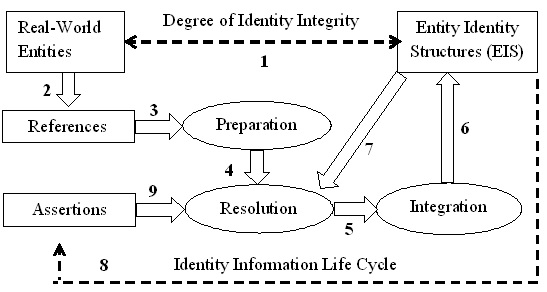
\includegraphics[width=14cm,height=7cm]{Figures/OriginalEIIM.jpg}
\end{figure} 

In this section we explain the current EIIM process that lays the foundation and acts as a background of the presented research.
The idea of Entity Identity Information Management (EIIM) as defined by [15] is the collection and management of identity information of real-world entities with the goal of sustaining entity identity integrity. Their model of EIIM was motivated by the problem of entity resolution in information systems, particularly in the domain of MDM (Master Data Management). They define entity resolution as the process of determining whether two references to real-world objects in an information system are referring to the same object, or to different object [16]. The EIIM life cycle as proposed by them is an iterative process that combines entity resolution and data structures representing entity identity into specific operational configurations (EIIM configurations, as shown in Figure 3), that when executed in concert, work to maintain the entity identity integrity of master data over time. The EIIM framework is implemented by developing open source software known as OYSTER .

